\chapter{Simulation comparison \& evaluations}
In the previous chapter we have described our model, with the reactive concession stratgey. Here the reactive concession strategy is compared to nonreactive concession strategy. Furthermore different values for the reservation utility are checked, and different values for the mixbed agent water requirements are seen. 

\section{Parameters}
The parameters that are checked are compared to the baseline nonreactive strategy. Firstly the Nash solution is described to compare to the optimal solution. 

\subsection{Nash Solution}
The Nash barganing solution is found using the product of the product of the is determined . It is pareto optimal \todo[cite (Nash 1950, Roth 1977, Lensberg 1988).]{cite (Nash 1950, Roth 1977, Lensberg 1988). Nash J (1950) The bargaining problem. Econometrica 18(2):155–162. Roth AE (1977) Individual rationality and Nash’s solution to the	bargaining problem. Math. Oper. Res. 2(1):64–65, Lensberg T (1988) Stability and the Nash solution. J. Econom. Theory 45(2):330–341.}
Our solution space is a convex set, as shown 

\begin{alignat*}{2}
\text{maximize }   	& \sum_{i=1}^m \log (u_i(x))  \\
\text{subject to \ } 	& u_i(x) \geq ru_i, & i = 1,...,m\\
& 0\leq x_j\leq 1, & j = 1,...,n\\
\end{alignat*}


NASH solution:
product of the 

\subsection{Nonreactive concession strategy}
As explained in \cref{sec:concessionstrat} the concession strategy used determines whether a solution will be found. If no concession is made during the negotiation, and the agent stay on their initial utility, no agreement can be made. In this result the nonreactive strategy used is as a base line to compare to other methods. As described, there are a large amount of different methods, and  here we decide on a weak concession, since the utiltiy functions of the other agents are unknown. The non reactive concession strategy used is $s_i(t) = \max \{s_0(t) - t * 0.01, ru_i\}$. This monotonic decreasing concession is a linear function until the reservation value. Described by \cite{wu2009efficient}, it is an \textit{amount of utility}, where Agent $ i \in N$ concedes a fixed amount utility $au$. Since the utility functions are private, utiliterian are not possible \citep{endriss2006monotonic}.

\subsection{Reactive Concession strategy}
The reactive concession strategy (see \cref{sec:reactiveconcessionstr} for an explanaition) is compared to the nonreactive. Similar to \citet{zheng2015automated}, however here different reservation utilities are checked.

\subsection{Reservation curve}
The curve, as shown in \cref{sec:design:negmod}, is not really a curve, but a linear solution. The values can differ from 	
reservation = [0.05, 0.10, 0.15,0.20,0.25,0.3,0.35, 0.4,0.45,0.5,0.55,0.6, 0.65];

\subsection{Threshold}
As shown in the algorithm \cref{al:algorithm1}, there is a threshold required to decide on the value and whether a converge is reached. For this simulation this is set to $\delta = 0.05$.	

\section{Reactive vs nonreactive}
When comparing the reactive to the nonreactive strategy, as shown in the graph, it is obvious that the nash limit indeed lies at 0.35...\todo[correct nash]{Correcte nash waarde toevoegen}. However, unexpectedly, the nonreactive strategy consequencly finds the solution closer to the optimal. However, this 

\begin{figure}
	\centering
	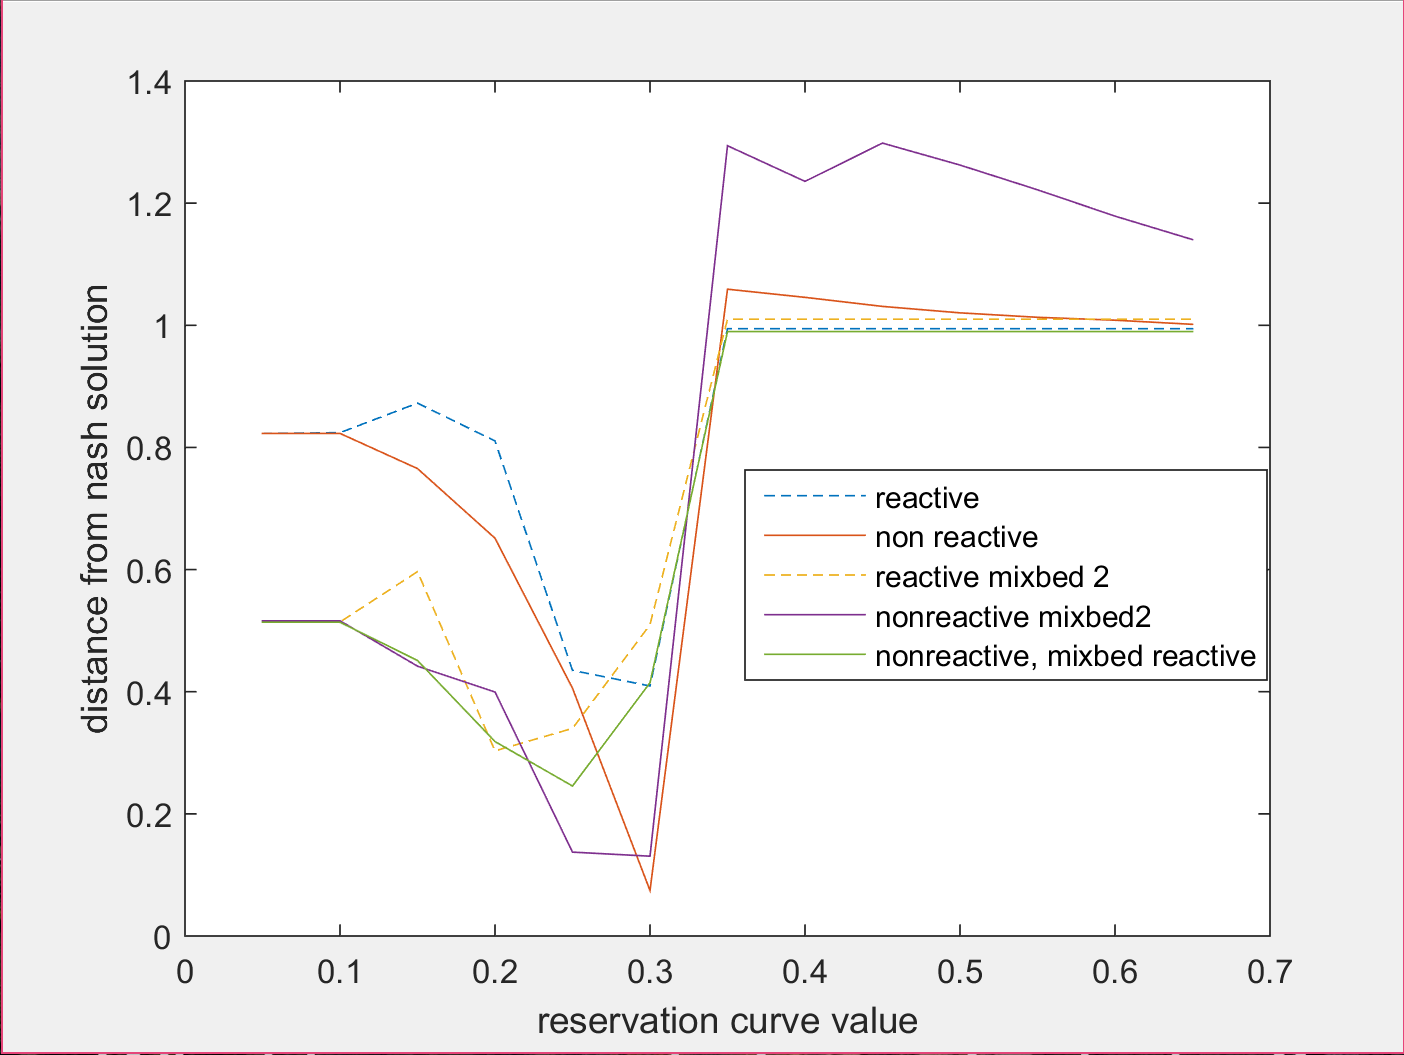
\includegraphics[width=0.7\linewidth]{img/all_dist_from_nash_solutions}
	\caption{All plots fromthe nash solutions.}
	\label{fig:alldistfromnashsolutions}
\end{figure}


The simaltation run is that of the Design

Mixbed water *2. The utility of water is a lot more important since the mixbed only has to clean a little.

Runnign the simulations:

for example. the solutions lay completely different. 


\citet{endriss2006monotonic} A concession should always be minimal with respect to the utility loss incurred by the agent making the concession.

\citet{endriss2006monotonic} Here some concession protocols are shown, \todo[explain monotonic multilateral concession protocols]{explain the multilateral concession protocols} however, since we are dealing with private information, this is not usefull. 


Agent anion and cation should form a front against the others, since they do not want water and mixbed is the only one wanting water.








%ARVO PÄRT Für Alina
%ARVO PÄRT Fratres
%PHILIP GLASS String Quartet No. 5
%STEVE REICH Different Trains












